\chapter{MAC Protocols}\label{sec:protocols}
In this section three contention-based \ac{mac} protocols are considered to handle the requirement of data transfers to physically close neighbours: a base case (ALOHA), a common approach (\ac{csma}) and a scenario specific approach (\ac{llbp}). 

\section{Considerations}\label{sec:mac_considerations}
Designing approaches so that as many radios as possible receive a transmission is of little help; from the receiver's perspective, if local-interest data is received 1500m away, the transmission is unwanted and increasing the chance of a local collision. To this end a criteria is defined as the maximum distance for which data is `wanted'; this is set to the worst-case transmission distance (500m).

The \ac{lora} configurations used are the abstracted \ac{dr}s from \ac{lorawan} \cite{3YP:LORAWAN_REGIONAL_PARAMS}; however, DR0 and DR2 are disregarded due to their lack of respective \ac{sf} performance. Although small packets ($< 20\enskip \text{bytes}$) have been shown to have slightly higher receive probability, they are not practical with transmission overhead, therefore packets are allowed to be any size ($\leq 255\enskip bytes$). \ac{cr} and \ac{tp}s are assumed to be 4/5 and 14dBm respectively.

As opposed to \ac{lorawan}'s \ac{dc} manager (see Figure \ref{fig:lorawan_duty_cycles}), all protocols use a custom \ac{dc} manager proposed in Appendix \ref{sec:proposed_duty_cycle}. This is  more flexible because it considers airtime over the full enforcement interval ($d_i$), allowing multiple sequential transmissions without silence; this is a requirement for bulk transmissions or protocol handshakes.

\section{Approaches}
\subsection{ALOHA}
Uses \ac{lorawan}'s principle of sending data periodically provided the \ac{dc} limit allows. No carrier-sensing is carried out, but transmissions will be delayed if the transmitter is receiving at the scheduled time. For purposes of testing, the minimum spacing between transmissions is that enforced by \ac{lorawan}. Therefore, in the case that any backoff occurs, less than the \ac{dc}'s maximum worth of data will be transmitted. \ac{mac} performance purely relies on each radio only using a small amount of airtime. As all radios must be on the same configuration the method can only use a single channel and \ac{dr} -- no mechanism is used for dynamically agreeing parameter changes. Consequently, a fixed \ac{dc} of up to 10\% is supported on band h1.6. Test packets use random payload sizes and all packets are treated as data.

\subsection{CSMA}
Uses the ALOHA approach but does carrier-sensing using \ac{lora}'s \ac{cad} process immediately before transmissions. On detection, random backoff will occur before the \ac{cad} process repeats; this is a simplified approach to that proposed in \cite{3YP:LORA_CSMA}. The \ac{ps}s are increased from 8 to 32 to increase preamble detection likelihood with the drawback of increased airtime overhead. When all nodes are within range of one another the vulnerable collision period is very short; provided no failed synchronisations take place, collisions should only occur if two transmitter's \ac{cad}s overlap; collisions resulting from the hidden node problem (Figure \ref{fig:hidden_node_problem}) are not avoided.

\begin{figure}[H]
    \centering
   	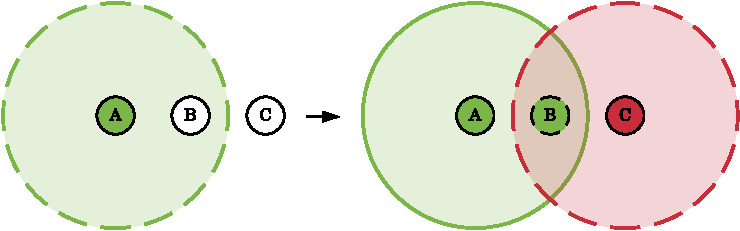
\includegraphics{Figures/hidden_node_problem}
    \caption[Demonstration of hidden node problem]{
    	Demonstration of the hidden node problem. A has transmitted before C, however, C was unable to sense A and assumes it is okay to transmit, resulting in a collision at B \cite{3YP:WSN_BOOK}.
    }
    \label{fig:hidden_node_problem}
\end{figure}


\subsection{LoRa Local Broadcast Protocol (\ac{llbp})}
This is a bespoke approach that makes use of dynamic channel and \ac{sf} switching with the target of constricting receivability to local listeners. The protocol uses two bands: a management-band (h1.4) and a data-band (h1.3). The former is treated as a single \ac{csma} channel, whereas the latter allocates 15 channels at \ac{cf}s $865.1 + 0.2 \cdot C_n$ (\ac{bw}=125kHz).

In principle, the protocol announces when a transmitter has a large chunk of data to send using a data announcement packet (\ac{dap}); this contains the \ac{lora} configuration to switch to and a description of the data being sent (Figure \ref{fig:dap_packet}). When a radio receives this packet it can make its own decision on whether it wants the data; if it does not it can ignore the message and will never see any data packets, otherwise it can switch configurations and only see those packets. This dump behaviour is heavily suited to \ac{scf} situations.

\begin{figure}[H]
    \centering
   	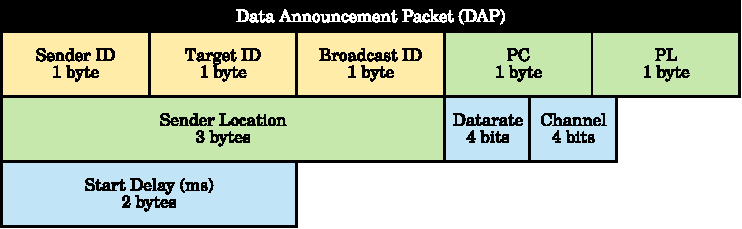
\includegraphics{Figures/dap}
    \caption[Data Announcement Packet (\ac{dap})]{
 		 \ac{dap} structure. The number of data packets being sent and their average length is provided so the receiver can timeout appropriately in case no packets arrive. The delay field is provided to indicate the relative start time to allow multiple \ac{dap}s. The target can be set to make announcements unicast.
    }
    \label{fig:dap_packet}
\end{figure}

As opposed to agreeing the configuration with a flurry of transmissions at one point, the configuration is decided by the transmitter, using its prior knowledge of surrounding transmitters. This knowledge is gained through periodical heartbeat packets (Figure \ref{fig:heartbeat_packet}), sent on the management-band; these provide \ac{snr}s and locations. The fastest viable \ac{dr} is picked along with a random data-band channel. There is no guarantee the channel is free but with the number of available channels, and a compulsory 1\% \ac{dc} across all of them, collisions are unlikely. \ac{dr} is selected such that for wanting receivers $\min(\text{\ac{snr}}) > (D_L + 2.5)$; this is where \ac{prp} should be approximately 100\%. The side effect of choosing the fastest \ac{dr} is less airtime; although this could be used to achieve more throughput, instead it is used to keep interference times to a minimum for the same data.

\begin{figure}[H]
    \centering
   	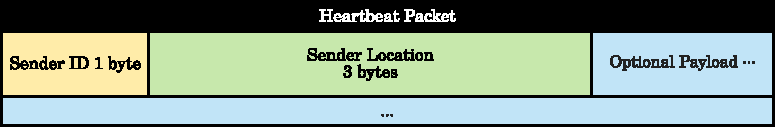
\includegraphics{Figures/heartbeat_packet}
    \caption[Heartbeat Packet]{
    	Heartbeat structure. Transmits a sender's location with \ac{snr} inferred. A payload can be attached to avoid wasted overhead.	
    }
    \label{fig:heartbeat_packet}
\end{figure}


\section{Test Methodology}
Protocol testing was executed on one of the simulator environment presets, \texttt{LargeData} \texttt{BroadcastTest}. The preset provided automatic generation of an $[x \times y]$ radio grid where spacing ($S$) was the same $\pm 20\%$. It provided four obstruction options seen in Figure \ref{fig:large_broadcast_options}.

\begin{figure}[H]
    \centering
   	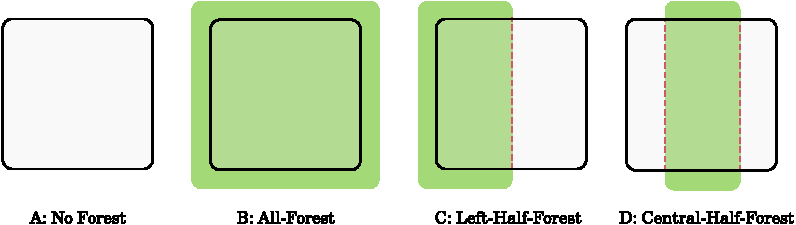
\includegraphics{Figures/test_environments}
    \caption[\texttt{LargeDataBroadcastTest} obstruction options]{
    	\texttt{LargeDataBroadcastTest} obstruction options, green indicates forest where $\beta = 0.55$. Radios are scattered in the black square
    }
    \label{fig:large_broadcast_options}
\end{figure}
If radios were always able to use their fastest configuration, it was unlikely a protocol with overhead would outperform one without. To alleviate this unfairness, $S$ was set to 400m; ensuring that in-forest radios needed \ac{dr}1 to communicate, but giving other transmissions the opportunity to increase \ac{dr}. 

The protocol configurations executed for each environment were:
\vspace{-5mm}
\begin{itemize}
\item ALOHA with \ac{dc}s of 1\% \textbf{[A]} and 10\% \textbf{[B]}.
\item CSMA with \ac{dc}s of 1\% \textbf{[C]} and 10\% \textbf{[D]}.
\item \ac{llbp} with \ac{dap} count of 1 \textbf{[E]} and 2 \textbf{[F]}.
\item \ac{llbp} with \ac{dap} count of 1 where true locations and \ac{snr} values were known \textbf{[G]}. This can be considered as \ac{llbp}'s best case performance but is not representative of actual performance. 
\end{itemize}
\vspace{-5mm}
For \ac{llbp} heartbeats were sent for 1/2 of the management-band airtime. 1/6th of the data-band airtime was sent after each \ac{dap}; meaning 6 \ac{dap}s an hour. Movement was not simulated but received heartbeats timed out after 10 minutes to reflect that movement is expected.

Each of the 28 configurations was executed in the simulator for 6 hours of simulation time, after which simulator statistics were exported.


\section{Results \& Discussion}
Each protocol is assessed by: its throughput of \textit{wanted} data per transmitter over the simulation period ($T$)  and the delivery percentage (DP). Together giving an understanding of the effective throughput. Aggregated results are seen in Figure \ref{tab:protocol_results} with separated box-plots of the two metrics in Figure \ref{fig:sim_throughput_boxplots} and Figure \ref{fig:sim_recv_boxplots} respectively.

\begin{table}[H]
\centering\small
\caption[Aggregated protocol testing results]{
Results aggregated by protocol, taking the mean of each transmitter across all environments. 
} 
\label{tab:protocol_results}
\renewcommand*{\arraystretch}{1.1}
\begin{tabular}{c|cc}
    \toprule
    \textbf{Configuration} & \makecell{Throughput (KB)} & DP (\%)  \\
    \midrule\addlinespace
    \textbf{A} & 35 & 91 \\
    \textbf{B} & 203 & 69 \\
    \textbf{C} & 30 & 91\\
    \textbf{D} & 183 & 77 \\
    \textbf{E} & 18 & 47 \\
    \textbf{F} & 34 & 52 \\
    \textbf{G} & 31 & 86 \\   
    \addlinespace\bottomrule
\end{tabular}
\end{table}

Unsurprisingly, throughputs are clustered by \ac{dc}, where $T_{10\%} \gg  T_{1\%}$. It could be expected that $10\times $ the \ac{dc} would result in $10\times $ the throughput; however the actual increase for both ALOHA and \ac{csma} is approximately $ 6\times$. The other $4\times $ accounted for by: backoff from the cluttered airspace ($\text{ALOHA}=1.9\times $, $\text{\ac{csma}}=2.5\times$), and more frequent failed/missed receives ($\text{ALOHA}=2.3\times $, $\text{\ac{csma}}=1.4\times$). Low DP, as a result of collisions and busy receivers, leads to unpredictability, increasing overhead caused by acknowledgements and retransmissions. The drops in DP for $\text{A}\rightarrow \text{B}$ and $\text{C}\rightarrow \text{D}$ are 22\% and 14\%. If these dropped packets require retransmissions, without considering acknowledgements, effective throughput drops to 47\% and 63\% respectively; considerations like these are implementation specific. Even given these arguments, effective throughput will usually improve by increasing \ac{dc} though more testing is required to find the limit. The 10\% drop in throughput and 8\% increase in DP for $\text{B}\rightarrow \text{D}$ indicates that \ac{csma} is only worth the overhead when taking retransmissions into account - if guaranteed receives are not required, ALOHA is more efficient.
%82 bytes 82 / 350 23.4%
%65 backoff 65 / 350 18.6\%
%42 bytes collisions 42 /300 14%
%75 backoff 75 / 300 = 25%
\vspace{10mm}
\begin{figure}[H]
    \centering
   	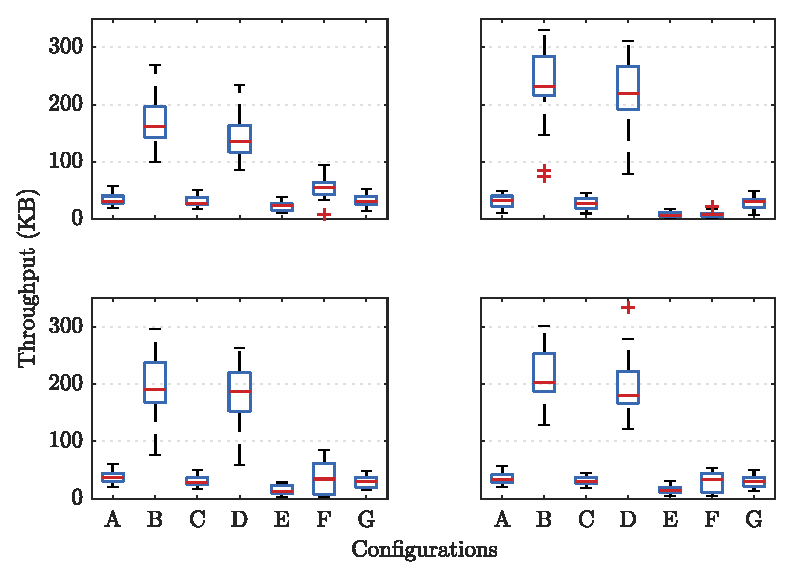
\includegraphics{Figures/sim_throughput_boxplots}
    \caption[Box-plots of protocol transmitter throughput]{
    	Box-plots of each transmitter's throughput in each environment [[A, B], [C, D]]. They demonstrate the throughput advantage of higher duty cycles and with that, higher variance between individual transmitter's access to the medium.}
    \label{fig:sim_throughput_boxplots}
\end{figure}

With this established, direct comparisons cannot be made between \ac{llbp} and configurations with 10\% \ac{dc}s. However, it is immediately clear that the \textit{fair} \ac{llbp} implementations do not out perform the 1\% ALOHA and \ac{csma} configurations; as is demonstrated by $P_{E || F} \ll P_{A||C}$ and $T_{E || F} \leq T_{A||C}$. Even with the best (\textit{cheat}) \ac{llbp} case, G has significantly less DP than the simpler approaches. Figure \ref{fig:sim_failure_reasons} indicates that the receiver can often not see data packets for \ac{llbp} configurations, indicating that the receiver does not switch bands correctly. This is likely caused by \ac{dap} receive failures; the theory made more likely by the significant increase of DP ($p = 0.01$) for $\text{E}\rightarrow \text{F}$. This issue is likely due to less critical heartbeat packets colliding with \ac{dap}s.
\newpage
 That being said, the far more significant problem can be seen by comparing E to G. G uses the same \ac{dap} count but has perfect data for \ac{dr} selection. The increase in performance indicates that transmitter decisions made by E/F are not informed by enough data, resulting in an overly aggressive \ac{dr}s being selected. These problems could be remedied by: increasing the heartbeat timeout, though this will slow down topology updates, or making heartbeats more frequent/descriptive, though this will increase \ac{dap} loss chance. To facilitate these changes the management-band could be switched to h1.6 (\ac{dr}=10\%), though this removes the possibility of having a separate high-rate channel for critical communications. 
\vspace{2cm}
\begin{figure}[H]
    \centering
   	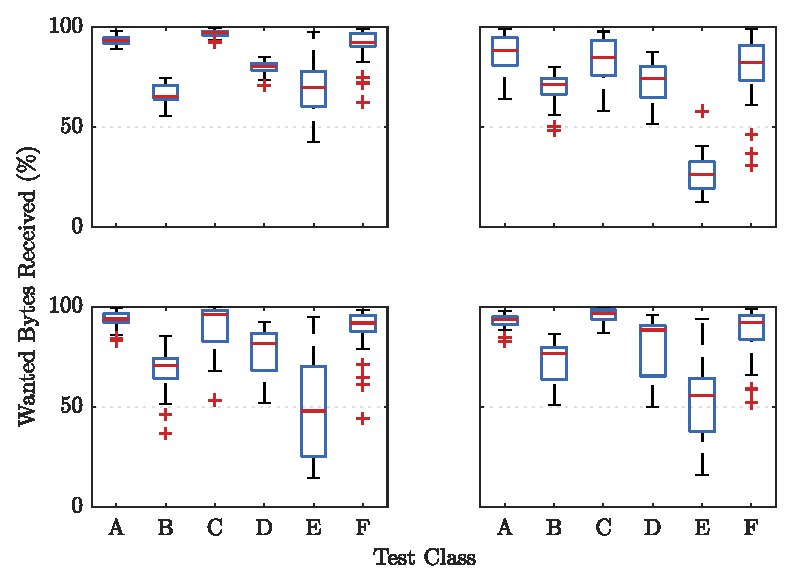
\includegraphics{Figures/sim_recv_boxplots}
    \caption[Box-plots of protocol data delivery percentage]{
    	Box-plots of DP in each environment [[A, B], [C, D]]. Highlighted is the consistency of ALOHA and \ac{csma} between environments. \ac{llbp}'s failings to select the correct \ac{dr} are highlighted by it only having acceptable performance in Environment A where any \ac{dr} will do.

    \label{fig:sim_recv_boxplots}
    }	
\end{figure}

\begin{figure}[H]
    \centering
   	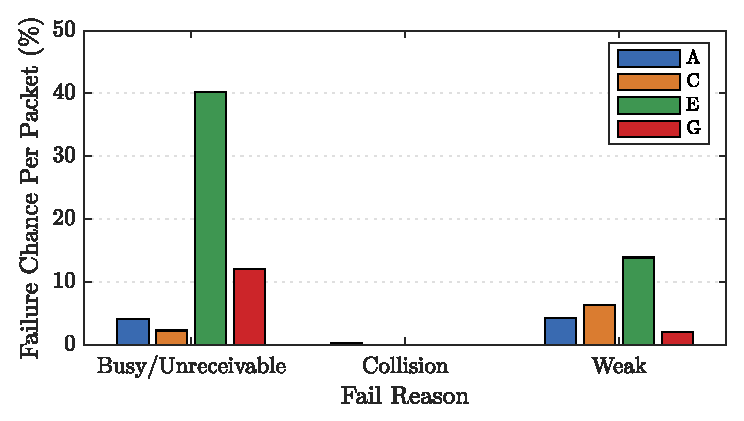
\includegraphics{Figures/sim_failure_reasons}
    \caption[Failure probabilities for protocol data packets]{
    Number of packet failures per configuration normalised by number of possible packet failures. Busy failures may have occurred due to the receiver: being synchronised with a stronger signal, doing CAD or being on the wrong configuration. Some collisions are recorded as weak due to general noise increases reducing demodulation success.
    \label{fig:sim_failure_reasons}
    }	
\end{figure}
